\documentclass[a4paper,12pt]{article}
\usepackage{HomeWorkTemplate}

\usepackage[utf8]{inputenc}
\usepackage[]{babel}

\setlength{\parindent}{4em}
\setlength{\parskip}{0.5em}

\renewcommand{\baselinestretch}{1.5}

\usepackage{caption}
\usepackage{subcaption}
\usepackage{float}
\usepackage{amsmath}
\usepackage[utf8]{inputenc}
\usepackage{lmodern, textcomp}
\usepackage{circuitikz}
\usepackage[shortlabels]{enumitem}
\usepackage{hyperref}
\usepackage{tikz}
\usepackage{amsmath}
\usepackage{amssymb}
\usepackage{tcolorbox}
\usepackage{graphicx}
\usepackage{xepersian}
\settextfont{XB Niloofar}
\usetikzlibrary{arrows,automata}
\usetikzlibrary{circuits.logic.US}
\usepackage{changepage}
\newcounter{problemcounter}
\newcounter{subproblemcounter}
\setcounter{problemcounter}{1}
\setcounter{subproblemcounter}{1}
\newcommand{\problem}[1]
{
	\subsection*{
		پرسش
		\arabic{problemcounter} 
		\stepcounter{problemcounter}
		\setcounter{subproblemcounter}{1}
		#1
	}
}
\newcommand{\subproblem}{
	\textbf{\harfi{subproblemcounter})}\stepcounter{subproblemcounter}
}


\begin{document}
	\handout
	{اصول پردازش تصویر}
	{دکتر مصطفی کمالی تبریزی}
	{نیم‌سال اول 1399\lr{-}1400}
	{اطلاعیه}
	{سیدعلیرضا خادم}
	{97100398}
	{تمرین سری سوم - سوال چهارم}
	زمان حدودی اجرا برای تصویر 4 برابر کوچک شده: 20 ثانیه
	\section*{موارد لازم.}
	برای اجرا لازم است تا تصویر
	\lr{birds.jpg}
	در مسیر
	\lr{EX3\_Q3/images/}
	قرار داشته باشد. همچنین در پیاده‌سازی این سوال از کتابخانه‌های 
	\lr{numpy}
	،
	\lr{skimage}
	و
	\lr{cv2}
	استفاده شده است که قبل از اجرا بایستی این کتابخانه‌ها روی سیستم شما نصب باشد.
	\section*{روند کلی حل.}
برای حل این سوال از روش 
\lr{felzenswalb \& huttenlocher}
استفاده شده است. کلیات این روش در اسلاید جلسه 16 آمده است اما مواردی که جزو مزیت‌های این روش محسوب می‌شود از قرار زیر است:
\begin{figure}[H]
	\centering
	\begin{subfigure}{0.6\textwidth}
		\centering
		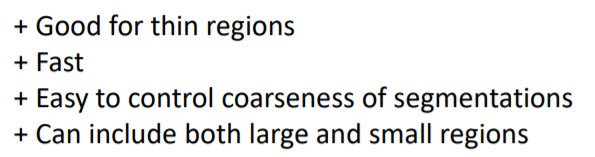
\includegraphics[width=\textwidth]{1.png}
	\end{subfigure}
\end{figure} 
	\section*{توضیح کد.}
	برنامه در مجموع حاوی 2 فایل با فرمت
	\lr{.py}
	می‌باشد که توضیحات هر فایل در پایین آمده است.
	\subsection*{$\circ$ utilities.py}
	\subsubsection*{\lr{resize\_image(src\_image, scale)}}
	این  تابع یک تصویر یک عدد (‌برحسب درصد) به بعوان ورودی می‌گیرد و طول و عرض تصویر را با نسبت داده شده تغییر می‌دهد و عکس تغییرسایز داده‌شده را به عنوان خروجی بر‌می‌گرداند.
	\subsubsection*{\lr{get\_num\_of\_clusters(segments)}}
	این تابع 
	\lr{segments}
	را به عنوان ورودی می‌گیرد و تعد کل سگمنت‌ها را به عنوان خروجی بر‌می‌گرداند.
	\subsubsection*{\lr{average\_color(src\_image, segments)}}
	این تابع یک تصویر و سگمنت‌های آن را به عنوان ورودی می‌گیرد و با پیمایش روی لیبل‌ها آن قسمت‌هایی از تصویر که به عنوان یک سگمنت هستند، رنگشان را با میانگین رونگ آن سگمنت جایگزین می‌کند.
	\subsubsection*{$\circ$ q4.py}
	در این فایل ابتدا تصویر 
	\lr{birds.jpg}
	را از مسیر
	\lr{EX3\_Q4/images/}
	لود می‌کنیم، بعد تصویر را به فضای 
	\lr{LAB}
	می‌بریم و آن را 4 برابر کوچک می‌کنیم. با استفاده روش 
	\lr{felzenswalb \& huttenlocher}
	که در کتابخانه 
	\lr{skimage.segmentation}
	پیاده‌سازی شده است 
	\lr{oversegmentation}
	را انجام می‌دهیم. تصویر سگمنت شده برای کاربر به نمایش در می‌آید تا یک پیکسل از پرنده‌ها را اتخاب کند. بعد از انتخاب یک پیکسل از پرنده‌ها توسط کاربر آن قسمت از تصویر را که با آن پیکسل در یک سگمنت قرار می‌گیرند را سفید می‌کنیم و نتیجه را با نام 
	\lr{res08.jpg}
	در مسیر
	\lr{EX3\_Q4/results/}
	ذخیره می‌کنیم.
	
	
\end{document}
